% Subespacios invariantes: autovalores y autovectores
% Números y figuras PNG: apunte/scripts/cap07_autovectores.py (uv run python apunte/scripts/cap07_autovectores.py)
\chapter{Subespacios invariantes: autovalores y autovectores}\label{cap:autovectores}

\section{La idea}

Imaginá una chapa fina de metal con una cuadrícula dibujada, que una prensa estira de manera
pareja: cada pedazo de la chapa se deforma igual que los demás, más en un sentido que en otro y
un poco de costado. Dos personas miran la misma chapa ya deformada. La primera sigue con la
vista una flecha dibujada y la ve más larga y apuntando a otro rumbo; sigue otra y le pasa lo
mismo, con otro largo y otro giro. ¿Qué regla puede haber detrás de tanto desorden?
La segunda persona se para mirando a lo largo de dos direcciones muy particulares, las únicas
en las que las flechas no giraron, y ve algo mucho más simple: la chapa se estiró por un factor
en una de esas direcciones y por otro factor en la otra. Nada más. ¿Cuál de las dos tiene
razón? Las dos miran lo mismo; la segunda eligió desde dónde mirar.

El capítulo~\ref{cap:subespacios} dejó dos herramientas: el determinante se anula cuando una
matriz aplasta alguna dirección, y el cuña de filas da esa dirección sin resolver sistemas;
ahora las usamos para encontrar, en cualquier matriz, las direcciones de la segunda persona: las
que la transformación no hace girar.
Pensá en una flecha que apuntaba al este: casi siempre sale apuntando a otro rumbo. Pero muchas
transformaciones tienen unas pocas direcciones privilegiadas en las que la flecha sale más
larga, más corta o dada vuelta, pero sobre la misma recta. Para qué nos sirven: esas rectas son
la estructura de la transformación; si las conocemos, sabemos qué hace la matriz sin mirar sus
números uno por uno.

Para decirlo con precisión hace falta un nombre para \enquote{un conjunto de vectores que la
matriz no saca de su lugar}. En la definición, \(W\) es un subespacio de \(\R^n\) (una recta o
un plano por el origen, o el espacio entero), \(A\) es la matriz que transforma y \(\lambda\)
(lambda) es el número por el que queda multiplicado un vector que no gira: el factor de
estiramiento de esa dirección.

\begin{definicion}[Subespacio invariante]\label{def:subespacio-invariante}
Un subespacio lineal \(W\subseteq\R^n\) es \emph{invariante} por la matriz \(A\) de
\(n\times n\) si \(Aw\in W\) para todo \(w\in W\): \(A\) lleva \(W\) dentro de sí mismo. Una
\emph{dirección invariante} es un subespacio invariante de dimensión \(1\), una recta
\(\{t\,v\}\) por el origen; que sea invariante quiere decir que \(Av\) es un múltiplo de
\(v\), \(Av=\lambda v\).
\end{definicion}

Los subespacios \(\{0\}\) y \(\R^n\) son invariantes por cualquier matriz; los interesantes
son los intermedios. ¿Cómo se ven en un caso concreto? Para la matriz
\(A=\left(\begin{smallmatrix}4&1\\2&3\end{smallmatrix}\right)\), la
figura~\ref{fig:autovec-grilla} muestra la cuadrícula deformada.
Probá primero con la flecha \((1,0)\): va a
\(A(1,0)^T=(4,2)^T\) y giró \(26{,}57^\circ\).
Probá ahora con \((1,1)\) y con \((1,-2)\): \(A(1,1)^T=(5,5)^T=5\,(1,1)^T\) y
\(A(1,-2)^T=(2,-4)^T=2\,(1,-2)^T\): sobre la recta de \((1,1)\) la matriz solo estira al
quíntuple, y sobre la de \((1,-2)\) solo al doble. ¿Tienen que ser perpendiculares esas dos
rectas? No tienen por qué: estas forman un ángulo de \(108{,}43^\circ\).

\begin{figure}[htbp]
\centering
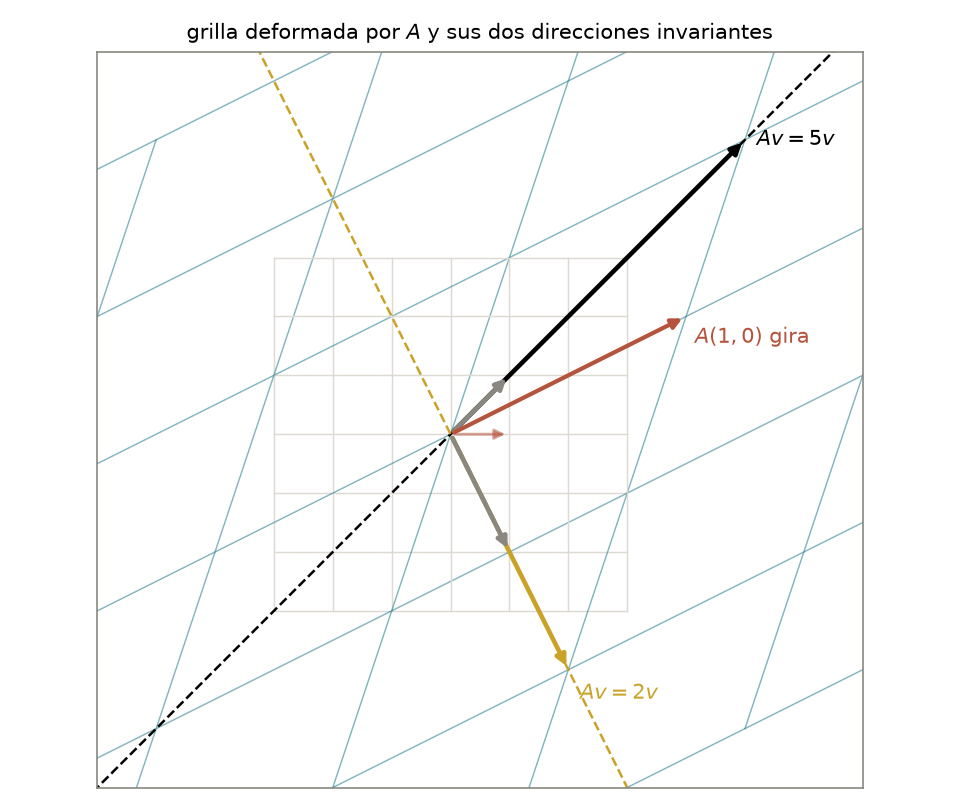
\includegraphics[width=.66\linewidth]{figuras/autovectores/autovec_grilla.png}
\caption{La grilla cuadrada (gris) deformada por
\(A=\left(\begin{smallmatrix}4&1\\2&3\end{smallmatrix}\right)\) (teal). Sobre la recta de
\((1,1)\) (negra) y la de \((1,-2)\) (dorada) la matriz solo estira, por \(5\) y por \(2\);
el vector \((1,0)\) (rojo) sale girado \(26{,}57^\circ\). Generada con
\texttt{apunte/scripts/cap07\_autovectores.py}.}
\label{fig:autovec-grilla}
\end{figure}

\begin{idea}[Una dirección invariante es una recta que la transformación no hace girar]
Los vectores que caen sobre su propia recta son los \emph{autovectores}, y el factor por el
que se estiran es el \emph{autovalor}. Conociendo dos autovectores independientes de una
matriz de \(2\times2\) y sus autovalores, la matriz queda determinada: todo vector se
descompone sobre esas dos rectas y cada componente se estira por su factor.
\end{idea}

Volvamos a las dos personas de la chapa, ahora con esta matriz. La segunda mide cada flecha por
cuántos pasos da sobre la recta de \((1,1)\) y cuántos sobre la de \((1,-2)\); para ella,
\(A\) solo multiplica la primera cantidad por \(5\) y la segunda por \(2\). Dicho como en el
capítulo~\ref{cap:cambio-base}: en la base de autovectores la matriz es diagonal, con los
autovalores en la diagonal y ceros fuera de ella. Te dejamos una pregunta para llevarte:
si en la base de autovectores la matriz es diagonal, ¿qué hace \(A\) aplicada cinco veces?
Pensalo con la figura (¿qué le pasa a una flecha de la recta de \((1,1)\) cada vez que se
aplica \(A\)?) antes de buscar la respuesta en el capítulo~\ref{cap:cambio-base}.

\unidadInteractiva{07b_nucleo_autovectores}{Núcleo y autovectores: las direcciones que no giran}{Explorá: elegí el caso «B = [[3, 1], [0, 2]]: dos direcciones, no perpendiculares» y mové la flecha de prueba hasta que \(v\) y \(Av\) queden alineados; después pasá a «corte [[1, 1], [0, 1]]» y a «giro de 30°» y contá cuántas direcciones quedan sin girar.}

\section{Construcciones, cuentas y ejemplos}

\subsection{Autovalores y autovectores}\label{sec:autovalores}

¿Cómo encuentra la segunda persona de «La idea» sus dos direcciones, si nadie se las marca en
la chapa? Probar flecha por flecha no termina nunca: hay infinitas direcciones. Lo que
necesitamos es una cuenta que diga, de una vez, cuáles son las flechas que no giran y cuánto se
estiran. Primero, los nombres.

Un \(v\neq0\) con \(Av=\lambda v\) es un \emph{autovector} de \(A\) con \emph{autovalor}
\(\lambda\) (definición~\ref{def:subespacio-invariante}). En coordenadas homogéneas eso dice
que la transformación deja fijo el punto que \(v\) representa.

\paragraph{El pase de magia.} La ecuación \(Av=\lambda v\) tiene dos incógnitas mezcladas,
el vector \(v\) y el número \(\lambda\). El truco es separarlas: primero buscamos los
\(\lambda\) posibles con una ecuación de una sola incógnita, y recién después, para cada uno,
su dirección. Con \(I\), la matriz identidad, \(Av=\lambda v\) equivale a \((A-\lambda I)\,v=0\):
\(v\) está en el núcleo de \(A-\lambda I\), y por la equivalencia de la
sección~\ref{sec:nucleo} ese núcleo no es trivial si y solo si
\[
  \boxed{\ \det(A-\lambda I)=0\ }\qquad\text{(polinomio característico)} .
\]
Buscamos los valores de \(\lambda\) para los que \(A-\lambda I\) aplasta alguna dirección:
el determinante, que el capítulo~\ref{cap:subespacios} usó para detectar matrices que aplastan,
ahora se usa como detector de autovalores.
Desarrollando el determinante quedan fórmulas cerradas en \(2\times2\) y en \(3\times3\):
\begin{gather*}
  \det\begin{pmatrix}a-\lambda&b\\c&d-\lambda\end{pmatrix}
  =\lambda^2-(\operatorname{tr}A)\,\lambda+\det A ,\\
  \det(A-\lambda I)=-\lambda^3+(\operatorname{tr}A)\,\lambda^2-c_2\,\lambda+\det A
  \qquad(3\times3),
\end{gather*}
donde \(c_2\) es la suma de los tres menores principales de \(2\times2\) (los que quedan al
tachar la fila y la columna \(i\), para \(i=1,2,3\)). Para la matriz de la sección
anterior, \(\operatorname{tr}A=7\) y \(\det A=10\): \(\lambda^2-7\lambda+10=(\lambda-5)(\lambda-2)\),
y aparecen los factores \(5\) y \(2\) de la figura~\ref{fig:autovec-grilla}.

¿Puede una matriz de \(3\times3\) no tener ninguna dirección que no gire? Pensá en una
rotación del espacio, por ejemplo un libro que gira sobre la mesa alrededor de un eje vertical:
casi todo gira, pero la dirección del eje se queda donde estaba. El polinomio dice que eso no es
casualidad.

\begin{resultado}[Cuántos autovalores reales]
Un polinomio real de grado \(3\) tiene tres raíces reales, o una real y dos complejas
conjugadas; nunca tres complejas, porque las raíces complejas de un polinomio real vienen de a
pares conjugados. A cada autovalor real le corresponde un autovector real; a uno complejo,
ningún vector de \(\R^3\). Una matriz de rotación de \(\R^3\) tiene siempre el autovalor \(1\),
cuyo autovector es el eje; los otros dos son \(e^{\pm i\theta}\), con \(\theta\) el ángulo de
giro, reales solo para \(\theta=0^\circ\) (identidad: \(1,1,1\)) y \(\theta=180^\circ\)
(\(1,-1,-1\)).
\end{resultado}

Encontrado un autovalor, falta su dirección. ¿Hay que resolver un sistema de ecuaciones? No
hace falta: alcanza con una cuenta que ya conocemos.

\begin{idea}[Método del producto cruz para el autovector]
Encontrado \(\lambda\), las filas de \(A-\lambda I\) son todas ortogonales al autovector.
Entonces el autovector es el producto vectorial de dos de esas filas:
\[
  v=(\text{fila}_i)\times(\text{fila}_j) .
\]
Si esas dos filas son paralelas y el producto da cero, se toma otro par. Si \emph{todos} los
pares dan cero, \(\operatorname{rango}(A-\lambda I)\le1\): el autoespacio tiene dimensión
\(\ge2\) (multiplicidad \emph{geométrica} \(\ge2\)) y hay al menos todo un plano de
autovectores (en homogéneas: toda una recta de puntos que no se mueven). La vuelta no vale: una raíz
doble del polinomio (multiplicidad \emph{algebraica} \(2\)) no garantiza que los pares se
anulen; ver el ejemplo~\ref{ej:autovec-cizalla} y la matriz 3a de la tabla de testigos del
capítulo~\ref{cap:cambio-base}. No hace falta resolver el sistema: es la misma operación de
\enquote{unir dos rectas en su punto común} de la sección~\ref{sec:vectorial},
y el producto cuña de filas con que se calculó el núcleo en el ejemplo~\ref{ej:nucleo-cuna}.
\end{idea}

\subsubsection{Ejemplo 1: reflexión respecto del plano \texorpdfstring{$xy$}{xy}}

Imaginá un espejo apoyado en el piso: ¿qué flechas se ven iguales en el reflejo y cuáles se
ven dadas vuelta? Las horizontales quedan como estaban; la vertical se invierte. La matriz de esa
reflexión, \(A=\operatorname{diag}(1,1,-1)\), conserva \(x,y\) e invierte \(z\):
\(\det(A-\lambda I)=(1-\lambda)^2(-1-\lambda)=0\) da \(\lambda=1\) (doble) y \(\lambda=-1\).
Para \(\lambda=-1\): \(A+I=\operatorname{diag}(2,2,0)\), y el producto cruz de las dos
primeras filas es \((2,0,0)\times(0,2,0)=(0,0,4)\): el eje \(z\), como se esperaba, con
\(A(0,0,4)^T=(0,0,-4)^T\). Para \(\lambda=1\): \(A-I=\operatorname{diag}(0,0,-2)\), y
cualquier par de filas da producto cruz nulo. Es la raíz doble: todo el plano \(xy\) es de
autovectores, porque la reflexión lo deja quieto punto a punto.

\subsubsection{Ejemplo 2: eje de una rotación compuesta}

Se compone una rotación de \(90^\circ\) alrededor de \(y\) seguida de una de \(90^\circ\)
alrededor de \(z\):
\[
  R=R_z(90^\circ)\,R_y(90^\circ)=
  \begin{pmatrix}0&-1&0\\1&0&0\\0&0&1\end{pmatrix}
  \begin{pmatrix}0&0&1\\0&1&0\\-1&0&0\end{pmatrix}
  =\begin{pmatrix}0&-1&0\\0&0&1\\-1&0&0\end{pmatrix}.
\]
Es una rotación, así que \emph{sin calcular el polinomio} se sabe que \(\lambda=1\) es
autovalor y que su autovector es el eje. Filas de \(R-I\): \((-1,-1,0)\), \((0,-1,1)\),
\((-1,0,-1)\). Producto cruz de las dos primeras: \((-1,-1,0)\times(0,-1,1)=(-1,1,1)\), y
\(R(-1,1,1)^T=(-1,1,1)^T\)~\(\checkmark\).
El eje es la dirección \((-1,1,1)\). Los otros autovalores son \(-\frac12\pm\frac{\sqrt3}2 i\):
un giro de \(120^\circ\) alrededor de ese eje. Con ángulos genéricos (por ejemplo
\(R_z(30^\circ)R_y(50^\circ)\)) la receta es idéntica y se hace en planilla o con una computadora: el
eje resulta \((-0{,}2263;\ 0{,}8446;\ 0{,}4853)\), y \(Rv=v\) se verifica multiplicando.

\begin{atencion}[Sobre los \enquote{números lindos}]
Los ejercicios de álgebra están diseñados para que den enteros. Una matriz genérica, como
la de una rotación de \(37^\circ\) o la homografía de un pentágono regular, da raíces
irracionales y autovalores con muchos decimales. Eso no es un error: es lo normal. Por eso
el método debe funcionar en planilla o en código, no solo a mano.
\end{atencion}

\subsection{En \texorpdfstring{$2\times2$}{2x2}: el autovector se lee en una fila}\label{sec:autovec-2x2}

¿Hace falta el producto cruz cuando la matriz es de \(2\times2\)? En el plano el producto cruz de dos filas no hace falta: si \(\lambda\) es autovalor,
\(A-\lambda I\) tiene determinante nulo y sus dos filas son paralelas (o nulas). Basta una
fila no nula \((a,b)\): el vector \((b,-a)\) es perpendicular a ella, y por lo tanto a las
dos, así que está en el núcleo. Es el cuña del plano del capítulo~\ref{cap:subespacios},
\(u\wedge v=u^\perp\cdot v\), leído al revés.

Mirá una elipse inclinada dibujada en una hoja. ¿Dónde están sus ejes, el más largo y el más
corto? A ojo se adivinan; con la ecuación de la elipse, el término cruzado los esconde. El
ejemplo siguiente muestra que los autovectores los encuentran sin medir nada.

\begin{ejemplo}[Una matriz simétrica y sus ejes principales]\label{ej:autovec-simetrica}
Sea \(S=\left(\begin{smallmatrix}5&2\\2&2\end{smallmatrix}\right)\). Con
\(\operatorname{tr}S=7\) y \(\det S=6\),
\(\det(S-\lambda I)=\lambda^2-7\lambda+6=(\lambda-6)(\lambda-1)\): \(\lambda_1=6\),
\(\lambda_2=1\).
Para \(\lambda_1=6\), \(S-6I=\left(\begin{smallmatrix}-1&2\\2&-4\end{smallmatrix}\right)\);
de la primera fila \((-1,2)\) sale \(v_1=(2,1)\), y en efecto \(S(2,1)^T=(12,6)^T=6\,(2,1)^T\).
Para \(\lambda_2=1\), \(S-I=\left(\begin{smallmatrix}4&2\\2&1\end{smallmatrix}\right)\); de
\((4,2)\) sale \((2,-4)\sim v_2=(1,-2)\), con \(S(1,-2)^T=(1,-2)^T\). Los dos autovectores
son perpendiculares: \((2,1)\cdot(1,-2)=0\). No es casualidad: \(S\) es simétrica
(sección~\ref{sec:simetricas}).

La curva \(x^TSx=5x^2+4xy+2y^2=1\) es una elipse con el término cruzado \(4xy\), que esconde
su orientación. Sus ejes están sobre los autovectores: sobre \(v_1\), a \(26{,}57^\circ\) del
eje \(x\), el semieje mide \(1/\sqrt{\lambda_1}=1/\sqrt6\approx0{,}408\); sobre \(v_2\),
\(1/\sqrt{\lambda_2}=1\) (figura~\ref{fig:autovec-elipse}). Control: \(6+1=7=\operatorname{tr}S\)
y \(6\cdot1=6=\det S\).
\end{ejemplo}

\begin{figure}[htbp]
\centering
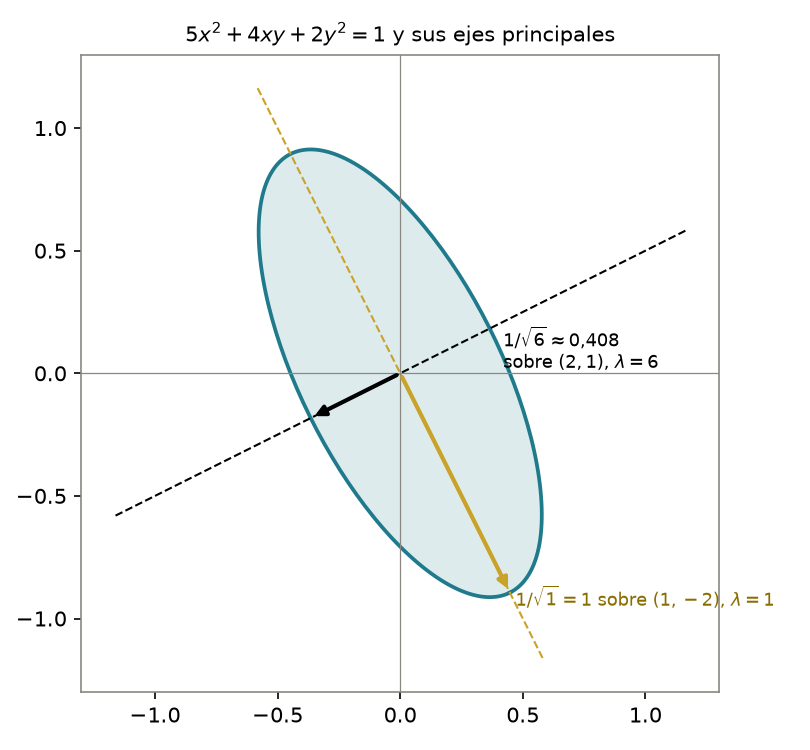
\includegraphics[width=.56\linewidth]{figuras/autovectores/autovec_elipse.png}
\caption{La elipse \(x^TSx=1\) con
\(S=\left(\begin{smallmatrix}5&2\\2&2\end{smallmatrix}\right)\). Sus ejes principales son
las direcciones de los autovectores \((2,1)\) y \((1,-2)\), perpendiculares; los semiejes
miden \(1/\sqrt6\approx0{,}408\) y \(1\). Generada con
\texttt{apunte/scripts/cap07\_autovectores.py}.}
\label{fig:autovec-elipse}
\end{figure}

Ahora tomá una pila de hojas sobre la mesa y empujá la de arriba de costado, sin levantarla:
cada hoja se corre en proporción a su altura. ¿Qué dirección no gira? Solo la horizontal, la de
las hojas mismas; cualquier otra flecha dibujada en el canto de la pila se inclina. A ese
movimiento lo llamamos corte (o cizalla), y el ejemplo muestra cómo se ve en el polinomio.

\begin{ejemplo}[Cizalla: autovalor doble con una sola dirección]\label{ej:autovec-cizalla}
Sea \(A=\begin{pmatrix}2&1\\0&2\end{pmatrix}\), una homotecia de razón \(2\) compuesta con un
corte horizontal. El polinomio es \(\lambda^2-4\lambda+4=(\lambda-2)^2\): un único
autovalor, \(\lambda=2\), doble. Pero
\(A-2I=\left(\begin{smallmatrix}0&1\\0&0\end{smallmatrix}\right)\) no es la matriz nula:
tiene rango \(1\), y su núcleo es solo la recta del eje \(x\), con \(A(1,0)^T=(2,0)^T\).
Cualquier otro vector gira hacia ese eje: \(A(0,1)^T=(1,2)^T\), \(A(1,1)^T=(3,2)^T\).
Comparemos con \(2I\), que tiene el mismo polinomio
\((\lambda-2)^2\) y para la cual \(2I-2I\) es nula, de rango \(0\): \emph{todas} las
direcciones son invariantes. El polinomio no distingue los dos casos; el rango de
\(A-\lambda I\), sí.
\end{ejemplo}

\subsection{Los cuatro casos en \texorpdfstring{$2\times2$}{2x2}}\label{sec:cuatro-casos}

Ya vimos una matriz con dos direcciones que no giran, una con todo un plano y una con una
sola. ¿Puede haber alguna sin ninguna? ¿Hay más posibilidades? En \(2\times2\) la respuesta
cabe en un número. El polinomio \(\lambda^2-(\operatorname{tr}A)\lambda+\det A\) tiene
discriminante \(\Delta=(\operatorname{tr}A)^2-4\det A\), el número que va dentro de la raíz en
la fórmula de la ecuación cuadrática, y su signo decide la geometría
(figura~\ref{fig:autovec-cuatro-casos}).

\begin{proposicion}[Clasificación de las matrices reales de \(2\times2\)]\label{prop:cuatro-casos}
Sea \(A\) real de \(2\times2\) y \(\Delta=(\operatorname{tr}A)^2-4\det A\).
\begin{enumerate}
  \item Si \(\Delta>0\), hay dos autovalores reales distintos y dos direcciones invariantes
  distintas.
  \item Si \(\Delta=0\) y \(A=\lambda I\), todo el plano es de autovectores.
  \item Si \(\Delta=0\) y \(A\neq\lambda I\), hay una sola dirección invariante.
  \item Si \(\Delta<0\), los autovalores son complejos conjugados y ninguna recta real es
  invariante.
\end{enumerate}
\end{proposicion}

\begin{demostracion}
Las raíces son \(\tfrac12\bigl(\operatorname{tr}A\pm\sqrt\Delta\bigr)\). Si \(\Delta>0\) son
dos reales distintas, cada una con un autovector, y los autovectores no pueden ser paralelos
porque un mismo \(v\) no se estira por dos factores distintos. Si \(\Delta<0\) son complejas
y no hay \(v\) real con \(Av=\lambda v\). Si \(\Delta=0\) hay una raíz doble \(\lambda\); si
\(A-\lambda I=0\) estamos en el caso 2, y si no, \(A-\lambda I\) tiene determinante nulo y una
fila no nula, rango \(1\), y su núcleo es una recta (caso 3).
\end{demostracion}

\begin{figure}[htbp]
\centering
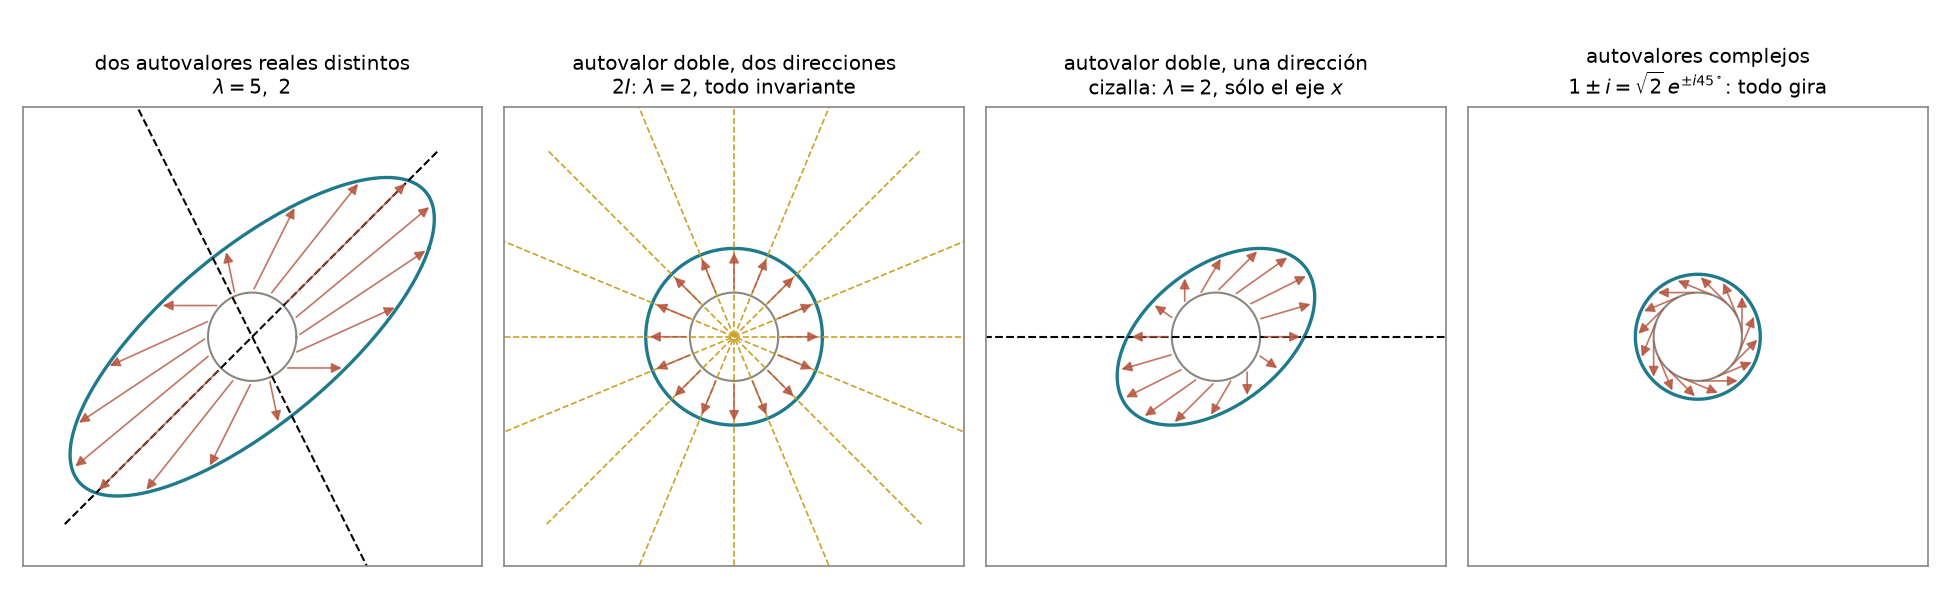
\includegraphics[width=\linewidth]{figuras/autovectores/autovec_cuatro_casos.png}
\caption{Los cuatro casos de la proposición~\ref{prop:cuatro-casos}: el círculo unidad
(gris), su imagen (teal) y la flecha de cada punto \(v\) a \(Av\) (rojo). De izquierda a
derecha:
\(\left(\begin{smallmatrix}4&1\\2&3\end{smallmatrix}\right)\), con \(\Delta=9\);
\(2I\) y la cizalla \(\left(\begin{smallmatrix}2&1\\0&2\end{smallmatrix}\right)\), ambas con
\(\Delta=0\); \(\left(\begin{smallmatrix}1&-1\\1&1\end{smallmatrix}\right)\), con
\(\Delta=-4\). Las rectas a trazos son las direcciones invariantes: sobre ellas la flecha es
radial. Generada con \texttt{apunte/scripts/cap07\_autovectores.py}.}
\label{fig:autovec-cuatro-casos}
\end{figure}

\paragraph{Autovalores complejos: una rotación con escala.} Si giramos el plano \(45^\circ\),
¿qué dirección queda sin girar? Ninguna, y el polinomio lo avisa con raíces complejas. La rotación \(R(\theta)\) del
capítulo~\ref{cap:rotaciones} tiene traza \(2\cos\theta\) y determinante \(1\), y
\(\lambda^2-2\cos\theta\,\lambda+1=0\) da \(\lambda=\cos\theta\pm i\sin\theta=e^{\pm i\theta}\).
Es la misma \(e^{i\theta}\) de la sección~\ref{sec:rot-complejos}: allí girar era multiplicar
por \(e^{i\theta}\), y acá ese número aparece como autovalor. Para \(\theta\neq0^\circ,
180^\circ\) el discriminante \(4\cos^2\theta-4\) es negativo y ninguna dirección real queda
sin girar, como debía ser. Una rotación con escala \(k\,R(\theta)\) tiene autovalores
\(k\,e^{\pm i\theta}\): el módulo es la escala y el argumento el ángulo. Por ejemplo,
\(\left(\begin{smallmatrix}1&-1\\1&1\end{smallmatrix}\right)=\sqrt2\,R(45^\circ)\) tiene
autovalores \(1\pm i=\sqrt2\,e^{\pm i45^\circ}\), de módulo \(1{,}4142\): todo vector gira
\(45^\circ\) y se alarga por \(\sqrt2\) (último panel de la
figura~\ref{fig:autovec-cuatro-casos}).

\subsection{En \texorpdfstring{$3\times3$}{3x3}: tres direcciones por cuña de filas}\label{sec:autovec-3x3}

En el espacio la receta es la misma, con un paso más: polinomio de grado \(3\), tres raíces y,
para cada una, el cuña de dos filas. Imaginá un bloque de goma que se estira distinto a lo largo
de tres direcciones: si las encontramos, describir la deformación del bloque es dar tres
números.

\begin{ejemplo}[Una matriz de \(3\times3\) con tres direcciones invariantes]\label{ej:autovec-3x3}
Sea \(M=\left(\begin{smallmatrix}2&1&0\\1&3&1\\0&1&2\end{smallmatrix}\right)\). Con
\(\operatorname{tr}M=7\), menores principales \(5\), \(4\), \(5\) (suma \(c_2=14\)) y
\(\det M=8\), el polinomio es
\(-\lambda^3+7\lambda^2-14\lambda+8=-(\lambda-1)(\lambda-2)(\lambda-4)\). Para cada
autovalor tomamos el cuña de las dos primeras filas de \(M-\lambda I\):
\begin{center}
\begin{tabular}{cccc}
\toprule
\(\lambda\) & filas 1 y 2 de \(M-\lambda I\) & cuña \(v\) & \(Mv\)\\
\midrule
\(1\) & \((1,1,0)\), \((1,2,1)\) & \((1,-1,1)\) & \((1,-1,1)\)\\
\(2\) & \((0,1,0)\), \((1,1,1)\) & \((1,0,-1)\) & \((2,0,-2)\)\\
\(4\) & \((-2,1,0)\), \((1,-1,1)\) & \((1,2,1)\) & \((4,8,4)\)\\
\bottomrule
\end{tabular}
\end{center}
La última columna confirma \(Mv=\lambda v\) en los tres casos. Las tres direcciones son
perpendiculares dos a dos (los tres productos internos dan \(0\)), porque \(M\) es simétrica,
y \(1+2+4=7=\operatorname{tr}M\), \(1\cdot2\cdot4=8=\det M\). En la base
\(\{(1,-1,1),(1,0,-1),(1,2,1)\}\) la matriz solo estira cada eje por su autovalor; ese cambio
de base es el tema del capítulo~\ref{cap:cambio-base}.
\end{ejemplo}

\subsection{Simulaciones}

\unidadInteractiva{07c_autovalores_3d_puntos_fijos}{Autovalores en 3D y puntos fijos proyectivos}{Verificá: con el caso «R\_z(θ) R\_y(90°)» y \(\theta=90^\circ\), comprobá que la única recta invariante es la de \((-1,1,1)\), el eje del ejemplo 2, y que los otros dos autovalores son complejos.}

Las cuentas del capítulo se comprueban con \texttt{apunte/scripts/cap07\_autovectores.py}; los
comandos para repetirlas en la computadora están al final de «En profundidad».

\section{En profundidad}

\subsection{Autovalores y geometría de una transformación}\label{sec:autovalores-geom}

Volvé a las afinidades del capítulo~\ref{cap:afines}: una banda elástica que se estira y se
inclina, y además se corre sobre la mesa. ¿Qué dicen los autovalores de su parte lineal, la
matriz \(A\) que deforma sin trasladar? Con otro nombre, lo mismo que en el plano: por dónde
estira sin girar.

\begin{definicion}[Dirección propia]\label{def:06-direccion-propia}
Una dirección \(d\neq0\) es \emph{propia} para la parte lineal \(A\) de una afinidad si
\(Ad=\lambda d\) para algún número \(\lambda\), el \emph{autovalor}. Es decir, \(d\) es un
autovector de \(A\). Los autovalores son las raíces de \(\det(A-\lambda I)=0\).
\end{definicion}

Sobre una dirección propia la afinidad solo estira, contrae o invierte; no gira. Con
\(\lambda=1\) la dirección no cambia; con \(\lambda=-1\) invierte su sentido; con
\(|\lambda|>1\) se expande y con \(0<|\lambda|<1\) se contrae. Con autovalores complejos no
hay direcciones propias reales: la parte lineal gira.

\begin{ejemplo}[Direcciones propias de la afinidad axial]\label{ej:06-autovalores-axial}
Para la afinidad axial del ejemplo~\ref{ej:06-axial}, \(A=\begin{pmatrix}1&1\\0&2\end{pmatrix}\)
y \(\det(A-\lambda I)=(1-\lambda)(2-\lambda)\). Los autovalores son \(1\) y \(2\):
\(A(1,0)^T=1\cdot(1,0)^T\) y \(A(1,1)^T=(2,2)^T=2\,(1,1)^T\). Las dos direcciones propias son la del eje (autovalor \(1\): el eje queda fijo) y la de
desplazamiento \(d=(1,1)\) (autovalor \(2\): la razón \(k\)). Los datos geométricos de la
construcción son los datos espectrales de la matriz. En cambio, en el
ejemplo~\ref{ej:06-rot-escala} los autovalores de \(A\) son \(0{,}354\pm0{,}354\,i\): no hay
direcciones propias reales porque la parte lineal gira \(45^\circ\).
\end{ejemplo}

En una rotación de \(\R^3\) el eje es una dirección propia de autovalor \(1\)
(capítulo~\ref{cap:rotaciones}); el mismo razonamiento, aplicado a la matriz homogénea bajo la
identificación afín natural \((x,y)\leftrightarrow(x,y,1)^T\) entre \(\R^2\) y el plano \(w=1\), localiza los
puntos fijos de una afinidad: los puntos que la afinidad deja en su lugar.

\begin{proposicion}[Punto fijo como autovector de autovalor 1]\label{prop:06-fijo-autovector}
Sea \(M=\begin{pmatrix}A&b\\0\ \ 0&1\end{pmatrix}\) la matriz homogénea de una afinidad. El
punto \(p\) es fijo si y solo si \((p,1)^T\) es autovector de \(M\) con autovalor \(1\). Un
autovector de autovalor \(1\) con última coordenada \(0\) no es un punto fijo, sino una
dirección propia de \(A\) con autovalor \(1\).
\end{proposicion}

\begin{demostracion}
Por bloques, \(M(p,1)^T=(Ap+b,\ 1)^T\). Esto es igual a \((p,1)^T\) si y solo si \(Ap+b=p\),
la definición de punto fijo. Si en cambio \(M(d,0)^T=(d,0)^T\), entonces \(Ad=d\). Un
autovector \((X,Y,W)^T\) con \(W\neq0\) se normaliza dividiendo por \(W\) y da el punto fijo
\((X/W,\ Y/W)\).
\end{demostracion}

En el ejemplo~\ref{ej:06-rot-escala}, los autovalores de \(M\) son \(0{,}354\pm0{,}354\,i\)
y \(1\), y el autovector de \(1\) normalizado es \((0{,}293;\ 0{,}293;\ 1)^T\): el punto que no se
mueve, \(p_\ast\).

\begin{idea}[Preguntas para leer una matriz afín]
¿Es invertible? Mirá \(\det A\). ¿Conserva la orientación? Mirá su signo. ¿Cómo cambian las
áreas? Por el factor \(|\det A|\). ¿Deja algún punto en su lugar? Resolvé \((I-A)p=b\), o buscá
autovectores de \(M\) de autovalor \(1\) con última coordenada no nula. ¿Tiene direcciones
invariantes? Buscá autovectores reales de \(A\).
\end{idea}

\subsection{Traza y determinante: suma y producto de los autovalores}\label{sec:traza-det-autovalores}

En todos los ejemplos se repitió el mismo control: la suma de los autovalores dio la traza y
el producto dio el determinante. ¿Casualidad de ejemplos elegidos con números lindos? No: es una
regla general, y engancha con el capítulo~\ref{cap:subespacios}, donde el determinante resultó
ser el factor por el que se multiplican las áreas.

\begin{proposicion}[Traza y determinante en función de los autovalores]\label{prop:traza-det}
Si \(\lambda_1,\dots,\lambda_n\) son los autovalores de \(A\) de \(n\times n\), contados con
su multiplicidad algebraica y aunque sean complejos, entonces
\[
  \lambda_1+\dots+\lambda_n=\operatorname{tr}A,\qquad
  \lambda_1\cdots\lambda_n=\det A .
\]
\end{proposicion}

\begin{demostracion}
Sea \(p(\lambda)=\det(A-\lambda I)\), el polinomio característico, de grado \(n\). Sus
raíces complejas, contadas con multiplicidad, son los autovalores, y su coeficiente
principal es \((-1)^n\), así que se factoriza como
\[
  p(\lambda)=(\lambda_1-\lambda)(\lambda_2-\lambda)\cdots(\lambda_n-\lambda)
  =(-1)^n\lambda^n+(-1)^{n-1}(\lambda_1+\dots+\lambda_n)\,\lambda^{n-1}+\dots+
  \lambda_1\cdots\lambda_n .
\]
Por otro lado, \(\det(A-\lambda I)\) es una suma de productos de \(n\) entradas de
\(A-\lambda I\), una de cada fila y de cada columna, con su signo. El producto de la
diagonal, \((a_{11}-\lambda)\cdots(a_{nn}-\lambda)\), aporta
\((-1)^n\lambda^n+(-1)^{n-1}(a_{11}+\dots+a_{nn})\lambda^{n-1}+\cdots\). Cualquier otro
producto deja afuera al menos dos entradas de la diagonal (si una entrada sale de la
diagonal en la fila \(i\), toma la columna de otra fila \(j\), que también tiene que salir de
la diagonal), así que tiene a lo sumo \(n-2\) factores con \(\lambda\) y no aporta a
\(\lambda^{n-1}\). Comparando el coeficiente de \(\lambda^{n-1}\),
\((-1)^{n-1}\operatorname{tr}A=(-1)^{n-1}(\lambda_1+\dots+\lambda_n)\). El término
independiente es \(p(0)=\det A\) por un lado y \(\lambda_1\cdots\lambda_n\) por el otro. En
\(2\times2\) queda la cuenta conocida:
\(\lambda^2-(\operatorname{tr}A)\lambda+\det A=(\lambda-\lambda_1)(\lambda-\lambda_2)\).
\end{demostracion}

La proposición tiene una lectura geométrica: \(\det A\) es el factor de área o de volumen
(proposición~\ref{prop:det-factor}), y sobre una base de autovectores la caja unidad se
estira por \(\lambda_1\) en un eje, por \(\lambda_2\) en otro, y así siguiendo; el volumen se
multiplica por el producto. Y da un atajo para las rotaciones de \(\R^3\): los autovalores
son \(1\), \(e^{i\theta}\) y \(e^{-i\theta}\), cuya suma es \(1+2\cos\theta\). Para la
rotación del ejemplo 2, \(\operatorname{tr}R=0\), de modo que \(\cos\theta=-\tfrac12\) y
\(\theta=120^\circ\), sin calcular ninguna raíz. Para \(2\times2\) con autovalores complejos
\(k\,e^{\pm i\theta}\), el producto es \(k^2=\det A\) y la suma \(2k\cos\theta=\operatorname{tr}A\).

\subsection{La traza como derivada del determinante}\label{sec:traza-derivada-det}

Imaginá un cuadrado de chapa que se estira apenas: un poco a lo ancho, otro poco a lo alto.
¿Cuánto creció el área? Casi la suma de los dos estiramientos relativos; lo que falta es el
producto de dos cantidades chicas, mucho más chico todavía. Esa suma es la traza.
Es otra lectura de la traza, que no necesita los autovalores: es lo que cambia el
determinante, el factor de área o de volumen (proposición~\ref{prop:det-factor}), cuando la
matriz se aparta un poco de la identidad. En la proposición, \(E\) es la matriz que dice cómo se
aparta, \(\varepsilon\) (épsilon) un número chico que mide cuánto, y \(O(\varepsilon^2)\)
reúne los términos que, al achicar \(\varepsilon\), se achican por lo menos como
\(\varepsilon^2\).

\begin{proposicion}[La traza es la derivada del determinante en la identidad]\label{prop:traza-derivada-det}
Sea \(E\) una matriz de \(n\times n\). Para \(\varepsilon\) pequeño,
\[
  \det(I+\varepsilon E)=1+\varepsilon\operatorname{tr}E+O(\varepsilon^2).
\]
En \(2\times2\) la igualdad es exacta con el término siguiente:
\(\det(I+\varepsilon E)=1+\varepsilon\operatorname{tr}E+\varepsilon^2\det E\).
\end{proposicion}

\begin{demostracion}
\emph{En \(2\times2\).} Con \(E=\left(\begin{smallmatrix}a&b\\c&d\end{smallmatrix}\right)\),
\[
  \det\begin{pmatrix}1+\varepsilon a&\varepsilon b\\ \varepsilon c&1+\varepsilon d\end{pmatrix}
  =(1+\varepsilon a)(1+\varepsilon d)-\varepsilon^2bc
  =1+\varepsilon(a+d)+\varepsilon^2(ad-bc).
\]
El término de orden \(\varepsilon\) sale solo del producto de la diagonal; las entradas
fuera de la diagonal aparecen multiplicadas entre sí y aportan a \(\varepsilon^2\).

\emph{En \(n\times n\).} Por inducción en \(n\); el caso \(n=1\) es
\(1+\varepsilon e_{11}\). Sea \(A=I+\varepsilon E\) y desarrollemos su determinante por
menores a lo largo de la primera fila:
\[
  \det A=(1+\varepsilon e_{11})\,M_{11}+\sum_{j\ge2}(-1)^{1+j}\,\varepsilon e_{1j}\,M_{1j},
\]
donde \(M_{1j}\) es el determinante que queda al quitar la fila \(1\) y la columna \(j\).
\(M_{11}=\det(I+\varepsilon E')\), con \(E'\) la matriz \(E\) sin su primera fila ni su
primera columna; por la hipótesis inductiva, \(M_{11}=1+\varepsilon\operatorname{tr}E'+
O(\varepsilon^2)\). Para \(j\ge2\), el menor \(M_{1j}\) conserva la fila \(j\) de \(A\) sin
su columna \(j\), es decir, sin el \(1\) de la diagonal: todas las entradas de esa fila son
de la forma \(\varepsilon e_{jk}\). Desarrollando \(M_{1j}\) por esa fila, cada término
lleva un factor \(\varepsilon\), así que \(M_{1j}=O(\varepsilon)\) y el término
\(\varepsilon e_{1j}M_{1j}\) es \(O(\varepsilon^2)\). Queda
\[
  \det A=(1+\varepsilon e_{11})\bigl(1+\varepsilon\operatorname{tr}E'\bigr)+O(\varepsilon^2)
  =1+\varepsilon\bigl(e_{11}+\operatorname{tr}E'\bigr)+O(\varepsilon^2)
  =1+\varepsilon\operatorname{tr}E+O(\varepsilon^2).
\]
Los términos de orden \(\varepsilon\) vienen solo de la diagonal: cualquier otro producto
del desarrollo usa por lo menos dos entradas fuera de ella.
\end{demostracion}

\paragraph{Lectura: el cambio relativo de área.} Si \(I+\varepsilon E\) actúa sobre una
figura de área \(S\), la imagen tiene área \(S\det(I+\varepsilon E)\), y el cambio
relativo es \(\Delta S/S=\det(I+\varepsilon E)-1=\varepsilon\operatorname{tr}E+O(\varepsilon^2)\).
A primer orden solo importa la diagonal de \(E\): \(\varepsilon e_{11}\) es el
estiramiento relativo en la dirección \(x\), \(\varepsilon e_{22}\) el de la dirección
\(y\), y los dos se suman. Una cizalla pura, con ceros en la diagonal, no cambia el área a
primer orden; lo mismo un giro pequeño. En \(\R^3\) vale igual para el volumen, con
\(\varepsilon(e_{11}+e_{22}+e_{33})\). La figura~\ref{fig:traza-area} lo muestra con
\(\varepsilon=0{,}1\) para tres matrices: con traza \(3\), el área medida es
\(1{,}3185\) frente a \(1+\varepsilon\operatorname{tr}E=1{,}3\); con traza \(0\) y una
cizalla, \(0{,}99\) frente a \(1\); con traza \(-3\), \(0{,}7225\) frente a \(0{,}7\). En
los tres casos la diferencia es exactamente \(\varepsilon^2\det E\) (\(0{,}0185\),
\(-0{,}01\) y \(0{,}0225\)), el término de segundo orden de la proposición.

\begin{figure}[htbp]
\centering
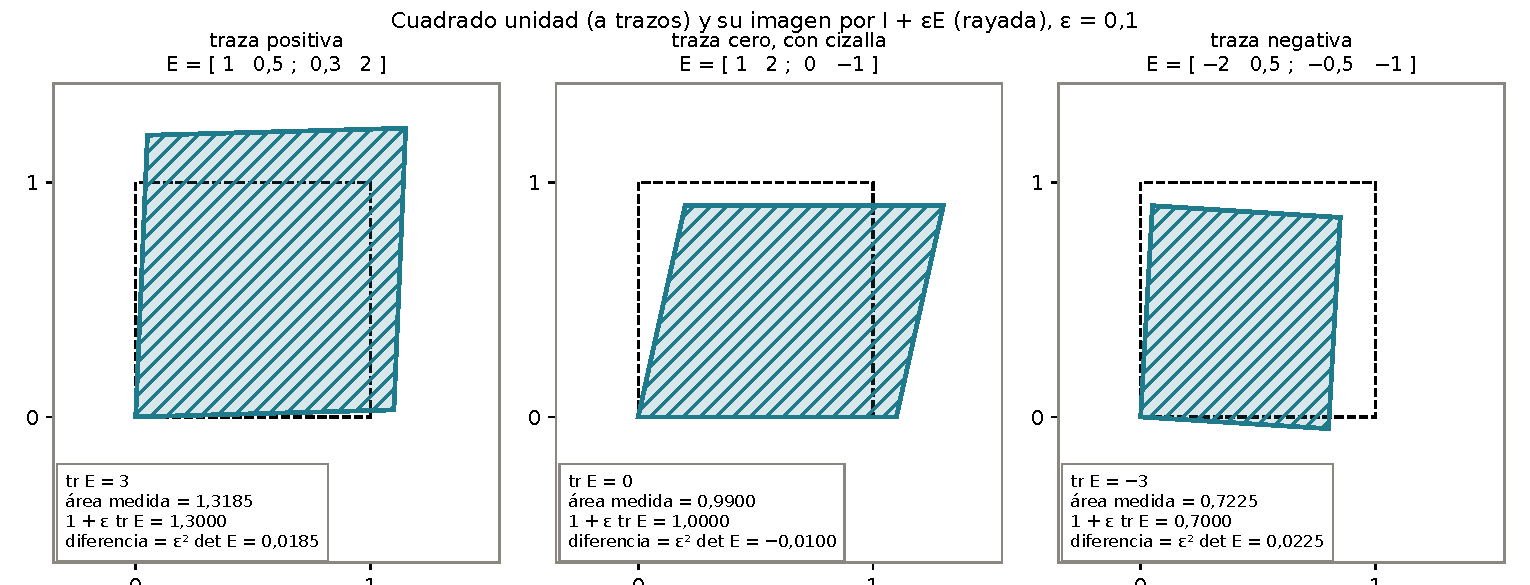
\includegraphics[width=\linewidth]{figuras/autovectores/cap07_traza_area.pdf}
\caption{El cuadrado unidad (a trazos) y su imagen por \(I+\varepsilon E\) (rayada), con
\(\varepsilon=0{,}1\), para \(E=\left(\begin{smallmatrix}1&0{,}5\\0{,}3&2\end{smallmatrix}\right)\)
(traza positiva), \(E=\left(\begin{smallmatrix}1&2\\0&-1\end{smallmatrix}\right)\) (traza
cero, con cizalla) y \(E=\left(\begin{smallmatrix}-2&0{,}5\\-0{,}5&-1\end{smallmatrix}\right)\)
(traza negativa). El área de la imagen, medida con la fórmula de Gauss
(proposición~\ref{prop:area-poligono}), se compara con \(1+\varepsilon\operatorname{tr}E\);
la diferencia es \(\varepsilon^2\det E\). Generada con
\texttt{apunte/scripts/cap07\_traza\_area.py}.}
\label{fig:traza-area}
\end{figure}

\paragraph{Otras lecturas de la traza.}
\begin{itemize}
\item \emph{Rotaciones.} En el plano,
\(\operatorname{tr}R(\theta)=2\cos\theta\), directamente de la matriz de rotación del
capítulo~\ref{cap:rotaciones}. En \(\R^3\), \(\operatorname{tr}R=1+2\cos\theta\)
(sección~\ref{sec:eje-exp} y sección~\ref{sec:traza-det-autovalores}): la traza da el
ángulo de giro sin calcular el eje. Una rotación pequeña es \(I+\varepsilon A\) con \(A\)
antisimétrica (proposición~\ref{prop:rot-pequenas}), de diagonal nula: \(\operatorname{tr}A=0\)
y, por la proposición~\ref{prop:traza-derivada-det}, el giro no cambia el área a primer
orden, como debe ser para una isometría.
\item \emph{Proyectores.} La traza de un proyector ortogonal es la dimensión del subespacio
sobre el que proyecta: \(\operatorname{tr}P=\operatorname{rango}P\)
(sección~\ref{sec:proyectores}). En una línea: de \(P^2=P\) y \(Pv=\lambda v\) sale
\(\lambda v=\lambda^2v\), así que los autovalores son \(0\) o \(1\); como \(P\) es
simétrica, por la proposición~\ref{prop:simetrica} hay una base ortonormal de autovectores,
y \(P\) conserva los de autovalor \(1\) y anula los demás, así que los primeros forman una base de la imagen; por la proposición~\ref{prop:traza-det}, la
traza cuenta esos unos. Para la recta por cuatro puntos del
ejemplo~\ref{ej:recta-cuatro-puntos}, \(\operatorname{tr}P=2\).
\item \emph{Valores singulares.} Para \(A\) de \(m\times n\),
\(\operatorname{tr}(A^TA)=\sum_i\lVert Ae_i\rVert^2=\sum_i\sigma_i^2\). La primera igualdad
es la definición: la entrada \(ii\) de \(A^TA\) es la columna \(i\) de \(A\) por sí misma,
\(\lVert Ae_i\rVert^2\). La segunda sale de que los \(\sigma_i^2\) son los autovalores de
\(A^TA\) (teorema~\ref{teo:svd-existencia}, capítulo~\ref{cap:svd}) y de la
proposición~\ref{prop:traza-det}. Para la matriz del ejemplo~\ref{ej:svd-mano},
\(\operatorname{tr}(A^TA)=9+16+25=50=45+5\).
\item \emph{Deformación.} La dilatación de una red es la traza del tensor de deformación
(sección~\ref{sec:aplicacion-deformacion}): es el caso \(n=2\) de la lectura de área de la
proposición~\ref{prop:traza-derivada-det}.
\end{itemize}

\begin{idea}[La traza suma lo que pasa en cada eje]
El determinante multiplica los factores de cada dirección; la traza los suma. Cerca de la
identidad las dos cuentas coinciden a primer orden.
\end{idea}

\subsection{Subespacios invariantes de dimensión 2: el plano de una rotación}\label{sec:plano-invariante}

Pensá en una puerta que gira sobre sus bisagras: ninguna flecha dibujada en la puerta conserva
su dirección, salvo la del eje de las bisagras, pero el plano en el que se mueve el picaporte
sigue siendo el mismo plano horizontal. Una matriz real sin autovalores reales no tiene rectas
invariantes, pero puede tener planos invariantes, y el autovector complejo los delata.

\begin{proposicion}[Plano invariante de un autovalor complejo]\label{prop:plano-invariante}
Sea \(A\) real de \(n\times n\) con un autovalor \(\lambda=\alpha+i\beta\), \(\beta\neq0\), y
autovector complejo \(u+iw\), con \(u,w\in\R^n\). Entonces el plano generado por \(u\) y
\(w\) es invariante por \(A\), y en él \(A\) actúa como una rotación con escala de módulo
\(|\lambda|\) en la base \(\{u,w\}\):
\[
  Au=\alpha u-\beta w,\qquad Aw=\beta u+\alpha w .
\]
\end{proposicion}

\begin{demostracion}
Desarrollando \(A(u+iw)=(\alpha+i\beta)(u+iw)\) queda
\(Au+i\,Aw=(\alpha u-\beta w)+i\,(\beta u+\alpha w)\).
Como \(A\), \(u\) y \(w\) son reales, se igualan partes reales e imaginarias, y quedan las dos
fórmulas. Ambas imágenes son combinaciones de \(u\) y \(w\), así que el plano que generan es
invariante. (Si \(u\) y \(w\) fueran paralelos, \(u+iw\) sería un múltiplo complejo de un
vector real \(r\), y \(Ar=\lambda r\) obligaría a \(\lambda\) a ser real.) La matriz
\(\left(\begin{smallmatrix}\alpha&\beta\\-\beta&\alpha\end{smallmatrix}\right)\) que queda es
\(|\lambda|\) por una rotación.
\end{demostracion}

En el plano, la rotación \(R(\theta)\) tiene autovector \((1,-i)\) para \(e^{i\theta}\): \(u=(1,0)\),
\(w=(0,-1)\), y el plano invariante es todo \(\R^2\). En el espacio, para la rotación del
ejemplo 2 los autovalores complejos tienen el plano invariante perpendicular al eje
\((-1,1,1)\), el plano \(-x+y+z=0\): el punto \(p=(1,1,0)\) de ese plano va a
\(Rp=(-1,0,-1)\), que vuelve a cumplir \(-(-1)+0+(-1)=0\). Toda rotación de \(\R^3\) se lee
así: una recta invariante (el eje, autovalor \(1\)) y un plano invariante perpendicular, donde
gira \(\theta\). Una rotación con escala del tipo
\(\left(\begin{smallmatrix}a&-b&0\\b&a&0\\0&0&c\end{smallmatrix}\right)\) tiene la misma
estructura con la escala \(\sqrt{a^2+b^2}\) en el plano \(xy\) y \(c\) sobre el eje \(z\).

\begin{idea}[Los subespacios invariantes son la anatomía de la matriz]
Una matriz real de \(3\times3\) se descompone siempre en piezas invariantes: tres rectas
(tres autovalores reales con tres autovectores independientes), o una recta y un plano
donde gira (un autovalor real y dos complejos), o, en los casos degenerados como la cizalla,
una recta y un plano invariantes que no se pueden partir en dos rectas. Calcular autovalores
es encontrar esas piezas.
\end{idea}

\subsection{Matrices simétricas: autovalores reales y direcciones perpendiculares}\label{sec:simetricas}

Los ejemplos~\ref{ej:autovec-simetrica} y~\ref{ej:autovec-3x3} dieron autovectores
perpendiculares, y las dos matrices eran simétricas (\(S^T=S\)). Las matrices simétricas
aparecen en todas partes: formas cuadráticas, las matrices que describen cómo se dispersan
los errores de medición, tensores de deformación. Su propiedad central es que nunca caen en los casos 3 y 4 de la
proposición~\ref{prop:cuatro-casos}. ¿Por qué una matriz que es igual a su transpuesta no
puede tener una sola dirección invariante, ni ninguna? La demostración es corta.

\begin{proposicion}[Autovalores y autovectores de una matriz simétrica]\label{prop:simetrica}
\begin{enumerate}
  \item Una matriz simétrica real de \(2\times2\) tiene sus dos autovalores reales, y solo
  pueden coincidir si es un múltiplo de \(I\).
  \item Si \(S\) es simétrica de \(n\times n\) y \(Sv_1=\lambda_1v_1\), \(Sv_2=\lambda_2v_2\)
  con \(\lambda_1\neq\lambda_2\), entonces \(v_1\cdot v_2=0\).
\end{enumerate}
\end{proposicion}

\begin{demostracion}
(1) Para \(S=\left(\begin{smallmatrix}a&b\\b&c\end{smallmatrix}\right)\),
\(\Delta=(a+c)^2-4(ac-b^2)=(a-c)^2+4b^2\ge0\), y vale \(0\) solo si \(a=c\) y \(b=0\), es
decir, si \(S=aI\).

(2) Usando \(x\cdot y=x^Ty\) y \(S^T=S\),
\[
  \lambda_1\,(v_1\cdot v_2)=(Sv_1)^Tv_2=v_1^TS^Tv_2=v_1^T(Sv_2)=\lambda_2\,(v_1\cdot v_2).
\]
Entonces \((\lambda_1-\lambda_2)(v_1\cdot v_2)=0\), y como \(\lambda_1\neq\lambda_2\),
\(v_1\cdot v_2=0\).
\end{demostracion}

El enunciado general, que en cualquier dimensión una simétrica tiene autovalores reales y una
base ortonormal de autovectores, se usa en el capítulo~\ref{cap:svd} como resultado.

\paragraph{La forma cuadrática en sus ejes principales.} Volvamos a la elipse inclinada del
ejemplo~\ref{ej:autovec-simetrica}: ¿por qué sus ejes caen justo sobre los autovectores? Sean \(u_1,u_2\) autovectores
unitarios y perpendiculares de la simétrica \(S\), con autovalores \(\lambda_1,\lambda_2\).
Escribiendo \(x=y_1u_1+y_2u_2\), con \(y_i=u_i\cdot x\),
\[
  x^TSx=(y_1u_1+y_2u_2)^T(\lambda_1y_1u_1+\lambda_2y_2u_2)=\lambda_1y_1^2+\lambda_2y_2^2,
\]
porque \(u_1\cdot u_2=0\) y \(u_i\cdot u_i=1\). En las coordenadas \(y_1,y_2\), medidas sobre
los autovectores, el término cruzado desapareció. Si \(\lambda_1,\lambda_2>0\), la curva
\(x^TSx=1\) es la elipse \(\lambda_1y_1^2+\lambda_2y_2^2=1\), de semiejes
\(1/\sqrt{\lambda_1}\) y \(1/\sqrt{\lambda_2}\) sobre \(u_1\) y \(u_2\): sus \emph{ejes
principales} (figura~\ref{fig:autovec-elipse}). El eje corto va con el autovalor grande. Si
un autovalor es negativo la curva es una hipérbola, con los mismos ejes. Esta lectura es la
base del capítulo~\ref{cap:svd}, donde la elipse viene de una matriz cualquiera a través de
\(A^TA\).

\subsection{Aplicación topográfica: deformación de una red de control entre dos épocas}\label{sec:aplicacion-deformacion}

Imaginá tres marcas fijadas en el suelo, a dos o tres kilómetros una de otra, cuya posición se
midió con mucho cuidado y se volvió a medir años después. Entre una medición y la otra las
marcas se corrieron unos centímetros. ¿Se corrió todo el terreno junto, como un bloque, o el
terreno se estiró?

\begin{idea}[Esto lo vas a usar en Topografía]
Una \emph{red de control} es un conjunto de puntos marcados en el terreno cuyas coordenadas se
conocen con mucha precisión y sirven de referencia para otras mediciones; cada campaña de
medición es una \emph{época}. Las coordenadas de la tabla son Gauss-Krüger, faja 5: un sistema
oficial de coordenadas planas en metros, con \(E\) creciendo hacia el este y \(N\) hacia el
norte. Son números largos, pero lo que importa son las diferencias. El \emph{acimut} de una
dirección es el ángulo que forma con el norte, contado en sentido horario.
\end{idea}

Tres puntos de una red de control se midieron en dos campañas, en esas coordenadas planas, en
metros. ¿Se deformó el terreno entre una época y otra? ¿Cuánto y en qué
direcciones?

\begin{center}
\small
\begin{tabular}{crrrrrr}
\toprule
punto & \(E\) época 1 & \(N\) época 1 & \(E\) época 2 & \(N\) época 2 & \(\Delta E\) (mm) & \(\Delta N\) (mm)\\
\midrule
\(P_1\) & \(5\,432\,118{,}437\) & \(6\,151\,874{,}215\) & \(5\,432\,118{,}405\) & \(6\,151\,874{,}170\) & \(-32\) & \(-45\)\\
\(P_2\) & \(5\,434\,602{,}881\) & \(6\,152\,593{,}062\) & \(5\,434\,602{,}924\) & \(6\,152\,593{,}100\) & \(43\) & \(38\)\\
\(P_3\) & \(5\,433\,041{,}590\) & \(6\,154\,210{,}774\) & \(5\,433\,041{,}615\) & \(6\,154\,210{,}757\) & \(25\) & \(-17\)\\
\bottomrule
\end{tabular}
\end{center}

Los desplazamientos, de \(55\), \(57\) y \(30\) mm, mezclan tres cosas: una traslación de todo
el bloque, un giro de todo el bloque y una deformación propiamente dicha. Solo la última
cambia distancias; los autovalores la separan.

\paragraph{La transformación afín exacta.} Buscamos una afinidad que lleve cada punto de la
época 1 a su posición en la época 2: \(F\) es su parte lineal, la matriz que deforma y gira, y
\(t\) el vector que traslada. Buscamos \(F\) de \(2\times2\) y \(t\) con
\(x_2=Fx_1+t\) para los tres puntos: \(6\) ecuaciones, \(6\) incógnitas. Conviene reducir al
baricentro de cada época, \(c_1=(5\,433\,254{,}3027;\ 6\,152\,892{,}6837)\) y
\(c_2=(5\,433\,254{,}3147;\ 6\,152\,892{,}6757)\). Restando el promedio de las tres
ecuaciones, \(c_2=Fc_1+t\), y queda \(x_2-c_2=F(x_1-c_1)\): la traslación se separa como el
desplazamiento del baricentro, \(c_2-c_1=(12{,}0;\ -8{,}0)\) mm, y \(F\) sale de las
coordenadas reducidas (en metros)
\[
  \begin{array}{c@{\qquad}c@{\qquad}c}
  & \text{época 1} & \text{época 2}\\[2pt]
  P_1 & (-1135{,}8657;\ -1018{,}4687) & (-1135{,}9097;\ -1018{,}5057)\\
  P_2 & (1348{,}5783;\ -299{,}6217) & (1348{,}6093;\ -299{,}5757)\\
  P_3 & (-212{,}7127;\ 1318{,}0903) & (-212{,}6997;\ 1318{,}0813)
  \end{array}
\]
Las tres reducidas de cada época suman cero, así que la de \(P_3\) es menos la suma de las
otras dos y no aporta información nueva: con \(P_1\) y \(P_2\),
\(F=[\,x_2^{(1)}\ x_2^{(2)}\,]\,[\,x_1^{(1)}\ x_1^{(2)}\,]^{-1}\), y \(P_3\) se cumple
solo. El resultado, escrito como desviación de la identidad, es
\[
  F-I=\begin{pmatrix}26{,}115&14{,}077\\33{,}805&-1{,}373\end{pmatrix}\cdot10^{-6}.
\]

\paragraph{Deformación y giro.} Toda matriz es suma de una parte simétrica y una
antisimétrica, \(F=\tfrac12(F+F^T)+\tfrac12(F-F^T)\). Para \(F\) cercana a \(I\), la parte
antisimétrica \(\left(\begin{smallmatrix}0&-\omega\\\omega&0\end{smallmatrix}\right)\) es un
giro pequeño de ángulo \(\omega\), que no cambia distancias, y la parte simétrica menos la
identidad es el \emph{tensor de deformación}
\[
  E=\tfrac12(F+F^T)-I=\begin{pmatrix}26{,}115&23{,}941\\23{,}941&-1{,}373\end{pmatrix}\ \mu\varepsilon,
  \qquad
  \omega=\tfrac12(F_{21}-F_{12})=9{,}864\cdot10^{-6}\ \text{rad}=2{,}035'' ,
\]
con \(1\ \mu\varepsilon\) (microstrain) \(=10^{-6}\), un milímetro por kilómetro. El bloque
giró \(2{,}035''\) en sentido antihorario (del Este hacia el Norte), además de deformarse.

\paragraph{Deformaciones y direcciones principales.} Es el momento de pararse donde se paraba
la segunda persona de «La idea»: en las dos direcciones en las que el terreno solo se estiró o
se acortó. \(E\) es simétrica: por la
proposición~\ref{prop:simetrica} tiene dos autovalores reales y autovectores perpendiculares.
Sus autovalores se llaman \emph{deformaciones principales} y, como en la tabla de notación
(sección~\ref{sec:notacion}), los escribimos \(e_1\) y \(e_2\) en lugar de \(\lambda\):
cada uno es el alargamiento relativo, en \(\mu\varepsilon\), sobre su dirección.
Con \(\operatorname{tr}E=24{,}742\ \mu\varepsilon\) y \(\det E=-609{,}021\ \mu\varepsilon^2\),
\[
  e_{1,2}=\tfrac12\operatorname{tr}E\pm\sqrt{\bigl(\tfrac12\operatorname{tr}E\bigr)^2-\det E}
  =12{,}371\pm27{,}606 ,
  \qquad
  e_1=39{,}977\ \mu\varepsilon,\quad e_2=-15{,}234\ \mu\varepsilon .
\]
El autovector de \(e_1\) es \((0{,}86541;\ 0{,}50107)\) en \((E,N)\), de acimut
\(59{,}93^\circ\): en esa dirección el terreno se estiró casi \(40\) mm por kilómetro. En la
perpendicular, de acimut \(149{,}93^\circ\), se acortó \(15{,}2\) mm por kilómetro
(figura~\ref{fig:autovec-red}). La \emph{dilatación}, cambio relativo de área, es la traza,
\(e_1+e_2=24{,}742\ \mu\varepsilon\); la \emph{cizalla máxima}, la mayor variación de ángulo
entre dos direcciones perpendiculares, es \(e_1-e_2=55{,}211\ \mu\varepsilon\).

Que la dilatación sea la traza se justifica con la proposición~\ref{prop:traza-derivada-det}:
toda figura de la red cambia su área por el factor \(\det F\), y en \(2\times2\)
\(\det F=\det\bigl(I+(F-I)\bigr)=1+\operatorname{tr}(F-I)+\det(F-I)\). La parte
antisimétrica tiene diagonal nula, así que \(\operatorname{tr}(F-I)=\operatorname{tr}E\), que
por la proposición~\ref{prop:traza-det} es \(e_1+e_2\). Con los números de la red,
\(\det F-1=24{,}742\ \mu\varepsilon\): el término de segundo orden,
\(\det(F-I)\approx-512\ \mu\varepsilon^2=-0{,}0005\ \mu\varepsilon\), no alcanza la tercera
cifra decimal.

\begin{figure}[htbp]
\centering
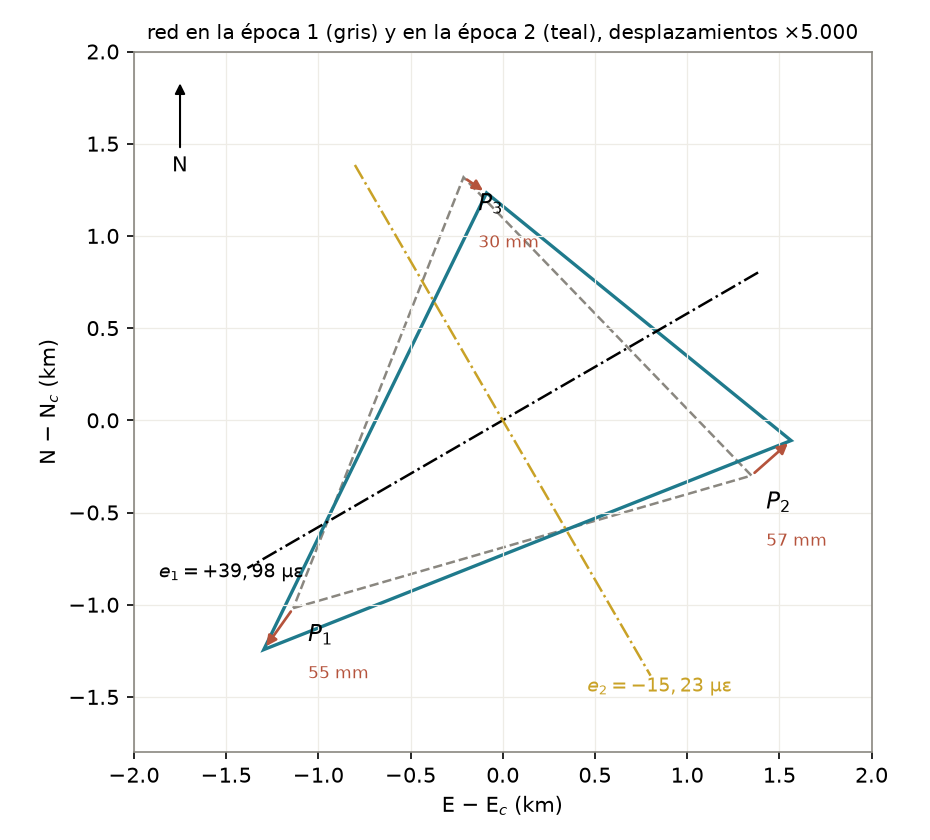
\includegraphics[width=.62\linewidth]{figuras/autovectores/autovec_red.png}
\caption{La red de control en la época 1 (gris, a trazos) y en la época 2 (teal), con los
desplazamientos multiplicados por \(5000\), y las direcciones principales de deformación:
estiramiento \(e_1=+39{,}98\ \mu\varepsilon\) a acimut \(59{,}93^\circ\) y acortamiento
\(e_2=-15{,}23\ \mu\varepsilon\) a acimut \(149{,}93^\circ\). Coordenadas reducidas al
baricentro, en km. Generada con \texttt{apunte/scripts/cap07\_autovectores.py}.}
\label{fig:autovec-red}
\end{figure}

\paragraph{Verificación con las distancias.} Para un lado de dirección unitaria \(u\), el
alargamiento relativo es, a primer orden, \(\Delta d/d\approx u^TEu\): el giro \(\omega\) no
interviene. Los tres lados lo confirman:
\begin{center}
\small
\begin{tabular}{crrrrrr}
\toprule
lado & \(d\) época 1 (m) & \(d\) época 2 (m) & \(\Delta d\) (mm) & acimut & \(\Delta d/d\) (\(\mu\varepsilon\)) & \(u^TEu\) (\(\mu\varepsilon\))\\
\midrule
\(P_1P_2\) & \(2586{,}3494\) & \(2586{,}4445\) & \(95{,}11\) & \(73{,}86^\circ\) & \(36{,}776\) & \(36{,}775\)\\
\(P_2P_3\) & \(2248{,}2486\) & \(2248{,}2215\) & \(-27{,}07\) & \(316{,}02^\circ\) & \(-12{,}042\) & \(-12{,}043\)\\
\(P_3P_1\) & \(2512{,}3136\) & \(2512{,}3605\) & \(46{,}99\) & \(201{,}56^\circ\) & \(18{,}702\) & \(18{,}702\)\\
\bottomrule
\end{tabular}
\end{center}
El lado \(P_1P_2\), que apunta a \(73{,}86^\circ\) del norte, está a solo \(14^\circ\) de la
dirección de \(e_1\) y se alargó casi tanto como permite \(e_1\); el lado \(P_2P_3\), que apunta
a \(316{,}02^\circ\) (o \(136{,}02^\circ\) en sentido contrario), está cerca de la dirección de
\(e_2\) y se acortó. Ningún lado puede alargarse más que \(e_1\) ni menos que \(e_2\): los
autovalores son el máximo y el mínimo de \(u^TEu\) sobre las direcciones unitarias.

\begin{atencion}[Tres puntos determinan la deformación, pero no la controlan]
Con tres puntos la transformación afín es exacta: no sobra ninguna ecuación y todo error de
medición pasa entero a \(E\). Un milímetro sobre \(2{,}5\) km son \(0{,}4\ \mu\varepsilon\);
deformaciones de ese orden no se distinguen del redondeo de las coordenadas. Con más puntos
el mismo planteo se resuelve por cuadrados mínimos: se elige la transformación que hace mínima la
suma de los cuadrados de lo que cada punto se aparta de ella. Esos apartamientos, los
\emph{residuos}, dan la precisión de \(E\) (ejercicio~\ref{ex:autovec-traza-area}).
\end{atencion}

\subsection{Las cuentas del capítulo en NumPy}

Para repetir las cuentas con NumPy, en la unidad o en el script del capítulo
(\texttt{cap07\_autovectores.py}, en la carpeta \texttt{apunte/scripts/}), alcanzan tres
comandos:
\begin{itemize}
\item \texttt{np.poly} da los coeficientes del polinomio característico;
\item \texttt{np.linalg.eig}, o \texttt{eigh} para simétricas, da autovalores y autovectores;
\item \texttt{np.cross} hace el cuña de filas.
\end{itemize}
Con ángulos genéricos, como en la rotación \(R_z(30^\circ)R_y(50^\circ)\) del ejemplo 2, la receta es la misma que a
mano; solo cambian los decimales.

\section{Ejercicios con solución}

\begin{ejercicio}\label{ex:autovec-2x2}
Hallá autovalores y autovectores de \(A=\begin{pmatrix}1&2\\3&2\end{pmatrix}\), verificá
traza y determinante, y describí qué hace \(A\) sobre cada dirección invariante.
\end{ejercicio}
\solucion{\(\det(A-\lambda I)=\lambda^2-3\lambda-4=(\lambda-4)(\lambda+1)\): \(\lambda_1=4\),
\(\lambda_2=-1\). Para \(4\), la fila \((-3,2)\) de \(A-4I\) da \(v_1=(2,3)\), con
\(A(2,3)^T=(8,12)^T=4\,(2,3)^T\). Para \(-1\), la fila \((2,2)\) de \(A+I\) da
\((2,-2)\sim v_2=(1,-1)\), con \(A(1,-1)^T=(-1,1)^T\). Control: \(4+(-1)=3=\operatorname{tr}A\)
y \(4\cdot(-1)=-4=\det A\). Sobre la recta de \((2,3)\), \(A\) estira al cuádruple; sobre la
de \((1,-1)\), invierte el sentido sin cambiar el largo. Como \(\det A<0\), \(A\) invierte la
orientación. Las dos direcciones no son perpendiculares (\(A\) no es simétrica).}

\begin{ejercicio}\label{ex:autovec-casos}
Clasificá según la proposición~\ref{prop:cuatro-casos} e indicá las direcciones invariantes
reales, si las hay: (a) \(\left(\begin{smallmatrix}3&-2\\1&1\end{smallmatrix}\right)\);
(b) \(\left(\begin{smallmatrix}3&1\\0&3\end{smallmatrix}\right)\);
(c) \(\left(\begin{smallmatrix}0&1\\1&0\end{smallmatrix}\right)\).
\end{ejercicio}
\solucion{(a) \(\operatorname{tr}=4\), \(\det=5\), \(\Delta=16-20=-4<0\): autovalores
\(2\pm i\), de módulo \(\sqrt5\approx2{,}236\) y argumento \(\pm26{,}565^\circ\). Ninguna
recta real es invariante; por la proposición~\ref{prop:plano-invariante}, en la base
\(\{u,w\}\) del autovector complejo la matriz es un giro de \(26{,}565^\circ\) con escala
\(\sqrt5\). (b) \(\operatorname{tr}=6\), \(\det=9\), \(\Delta=0\): \(\lambda=3\) doble, y
\(A-3I=\left(\begin{smallmatrix}0&1\\0&0\end{smallmatrix}\right)\neq0\) tiene rango \(1\):
una sola dirección, el eje \(x\) (es una cizalla, caso 3). (c) \(\operatorname{tr}=0\),
\(\det=-1\), \(\Delta=4>0\): \(\lambda=\pm1\), con \((1,1)\) para \(1\) y \((1,-1)\) para
\(-1\): la reflexión respecto de la recta \(y=x\), que deja quieta esa recta e invierte su
perpendicular.}

\begin{ejercicio}\label{ex:autovec-rotacion}
Sea \(R=R_x(90^\circ)\,R_z(90^\circ)\). Calculá \(R\), su eje por cuña de filas de \(R-I\)
y el ángulo de giro usando la traza.
\end{ejercicio}
\solucion{\(R_z(90^\circ)=\left(\begin{smallmatrix}0&-1&0\\1&0&0\\0&0&1\end{smallmatrix}\right)\),
\(R_x(90^\circ)=\left(\begin{smallmatrix}1&0&0\\0&0&-1\\0&1&0\end{smallmatrix}\right)\) y
\(R=\left(\begin{smallmatrix}0&-1&0\\0&0&-1\\1&0&0\end{smallmatrix}\right)\). Filas de
\(R-I\): \((-1,-1,0)\), \((0,-1,-1)\), \((1,0,-1)\). El cuña de las dos primeras es
\((-1,-1,0)\times(0,-1,-1)=(1,-1,1)\), y \(R(1,-1,1)^T=(1,-1,1)^T\): el eje es la dirección
\((1,-1,1)\). Como \(\operatorname{tr}R=0=1+2\cos\theta\), \(\cos\theta=-\tfrac12\) y
\(\theta=120^\circ\); los otros dos autovalores son \(e^{\pm i\,120^\circ}\) y el plano
\(x-y+z=0\), perpendicular al eje, es invariante.}

\begin{ejercicio}\label{ex:autovec-elipse}
Hallá los ejes principales, los semiejes y el área de la elipse \(3x^2+2xy+3y^2=1\).
\end{ejercicio}
\solucion{La forma es \(x^TSx\) con \(S=\left(\begin{smallmatrix}3&1\\1&3\end{smallmatrix}\right)\)
(el coeficiente \(2\) del término cruzado se reparte en dos entradas iguales a \(1\)).
\(\det(S-\lambda I)=\lambda^2-6\lambda+8=(\lambda-4)(\lambda-2)\). Para \(\lambda=4\), la fila
\((-1,1)\) de \(S-4I\) da \((1,1)\); para \(\lambda=2\), la fila \((1,1)\) de \(S-2I\) da
\((1,-1)\): los ejes son las diagonales, perpendiculares. Semiejes: \(1/\sqrt4=0{,}5\) sobre
\((1,1)\) y \(1/\sqrt2\approx0{,}7071\) sobre \((1,-1)\). Área: \(\pi\cdot0{,}5\cdot0{,}7071
=\pi/\sqrt{\det S}=\pi/\sqrt8\approx1{,}1107\).}

\begin{ejercicio}\label{ex:autovec-deformacion}
En una zona se estimó el tensor de deformación (primera coordenada Este, segunda Norte)
\(E=\left(\begin{smallmatrix}30&10\\10&-10\end{smallmatrix}\right)\ \mu\varepsilon\). Hallá
las deformaciones principales, sus acimutes, la dilatación, la cizalla máxima y cuánto cambió
una base de \(1500\) m orientada al Norte.
\end{ejercicio}
\solucion{\(\operatorname{tr}E=20\), \(\det E=-300-100=-400\):
\(e_{1,2}=10\pm\sqrt{100+400}=10\pm\sqrt{500}\), es decir \(e_1=32{,}361\ \mu\varepsilon\) y
\(e_2=-12{,}361\ \mu\varepsilon\). La primera fila de \(E-e_1I\) es \((-2{,}361;\ 10)\), y su
perpendicular \((10;\ 2{,}361)\) es la dirección de \(e_1\): acimut
\(\arctan(10/2{,}361)=76{,}72^\circ\). La de \(e_2\) es la perpendicular, de acimut
\(166{,}72^\circ\). Dilatación \(e_1+e_2=20\ \mu\varepsilon\); cizalla máxima
\(e_1-e_2=2\sqrt{500}\approx44{,}721\ \mu\varepsilon\). Para la base Norte, \(u=(0,1)\) y
\(u^TEu=E_{22}=-10\ \mu\varepsilon\): se acortó \(10^{-5}\cdot1500\ \text{m}=15\) mm.}

\begin{ejercicio}\label{ex:autovec-traza-area}
Cuatro puntos de una red local, en coordenadas planas \((E,N)\) en metros, se midieron en
dos épocas. En la época 1 son \(P_1=(1000;\ 1000)\), \(P_2=(3400;\ 1200)\),
\(P_3=(3000;\ 3300)\) y \(P_4=(1200;\ 2900)\), y entre épocas se desplazaron
\((39;\ -4)\), \((84;\ -11)\), \((95;\ 3)\) y \((60;\ 8)\) mm. (a) Con cuatro puntos no hay
una transformación afín exacta: ajustá \(F-I\) por mínimos cuadrados, con coordenadas
reducidas al baricentro, y calculá los residuos. (b) Calculá \(\operatorname{tr}E\).
(c) Calculá el área del cuadrilátero \(P_1P_2P_3P_4\) en las dos épocas con la fórmula de
Gauss (sección~\ref{sec:poligono-cunas}) y compará el cambio relativo de área con
\(\operatorname{tr}E\).
\end{ejercicio}
\solucion{Se usan los cuatro puntos con mínimos cuadrados, y no tres con el cuarto de
control, para que todos pesen igual; los residuos hacen de control.
(a) Baricentro de la época 1: \((2150;\ 2100)\) m; desplazamiento medio
\((69{,}5;\ -1{,}0)\) mm, que es la traslación. Coordenadas reducidas \(x_i\):
\((-1150;\ -1100)\), \((1250;\ -900)\), \((850;\ 1200)\), \((-950;\ 800)\) m;
desplazamientos reducidos \(\delta_i\): \((-30{,}5;\ -3)\), \((14{,}5;\ -10)\),
\((25{,}5;\ 4)\), \((-9{,}5;\ 9)\) mm. El modelo es \(\delta_i=(F-I)\,x_i\), y cada fila de
\(F-I\) se ajusta por separado con las ecuaciones normales
(proposición~\ref{prop:ecuaciones-normales}, capítulo~\ref{cap:inversas}), con la misma
matriz \(X\) de filas \(x_i\):
\(X^TX=\left(\begin{smallmatrix}4\,510\,000&400\,000\\400\,000&4\,100\,000\end{smallmatrix}\right)\)
m\(^2\), \(X^T\delta_E=(83\,900;\ 43\,500)\) y \(X^T\delta_N=(-14\,200;\ 24\,300)\) m\(\cdot\)mm.
Resolviendo, en mm/km, o sea en \(\mu\varepsilon\),
\(F-I=\left(\begin{smallmatrix}17{,}8163&8{,}8716\\-3{,}7063&6{,}2884\end{smallmatrix}\right)\
\mu\varepsilon\).
Los residuos \(\delta_i-(F-I)x_i\) no superan \(0{,}45\) mm.
(b) La parte antisimétrica tiene diagonal nula, así que
\(\operatorname{tr}E=\operatorname{tr}(F-I)=17{,}8163+6{,}2884=24{,}105\ \mu\varepsilon\).
(c) \(S_1=4\,230\,000\) m\(^2\). Sumando los desplazamientos a las coordenadas (en metros,
con los milímetros) y aplicando otra vez la fórmula, \(S_2=4\,230\,101{,}9006\) m\(^2\):
\(\Delta S=101{,}90\) m\(^2\) y \(\Delta S/S_1=24{,}090\ \mu\varepsilon\). La
proposición~\ref{prop:traza-derivada-det} predice \(\operatorname{tr}E=24{,}105\
\mu\varepsilon\), es decir \(101{,}96\) m\(^2\); el término de segundo orden es despreciable
(\(\det F-1\) también da \(24{,}105\ \mu\varepsilon\)). La diferencia, \(0{,}015\
\mu\varepsilon\) o \(0{,}06\) m\(^2\), se debe a que el cuadrilátero de la época 2 no es
exactamente la imagen afín del de la época 1: es la huella de los residuos de
\(0{,}45\) mm como máximo. Cien metros cuadrados parecen mucho, pero repartidos sobre un
perímetro de \(8\,300\) m equivalen a que los lados se corran hacia afuera, en promedio,
\(12\) mm.}

\begin{ejercicio}\label{ex:autovec-rotacion-so3}
Sea \(R\in SO(3)\) una rotación distinta de la identidad. Demostrá que \(\lambda=1\) es
autovalor de \(R\) y que su autovector es la dirección del eje de rotación.
\end{ejercicio}
\solucion{Al ser \(R\) una matriz real de dimensión impar, su polinomio característico tiene
al menos una raíz real. Como \(R\) es ortogonal, todo autovalor tiene módulo \(1\), así que el
autovalor real es \(1\) o \(-1\). Los otros dos, si no son reales, forman un par conjugado
\(e^{i\theta},e^{-i\theta}\) de producto \(1\); como \(\det R=1\), el autovalor real restante
es \(\lambda=1\). Su autovector es la dirección del eje de rotación. Se excluye \(R=I\) porque
en la identidad todos los vectores son propios con autovalor \(1\) y no hay un eje
distinguido.}

\begin{ejercicio}\label{ex:autovec-ortogonal-det-negativo}
Decidí si es cierto que toda matriz ortogonal de \(\R^3\) con determinante \(-1\) tiene tres
autovalores reales iguales a \(1\) o \(-1\).
\end{ejercicio}
\solucion{No es cierto en general. Por ser real y de dimensión impar, la matriz tiene al menos
un autovalor real; por ser ortogonal, sus autovalores tienen módulo \(1\), y por tener
determinante \(-1\) siempre existe el autovalor \(\lambda=-1\). Los otros dos pueden ser
\(e^{\pm i\theta}\), que no son reales cuando \(\theta\notin\{0,\pi\}\). Geométricamente es una
\emph{rotorreflexión}: una rotación en un plano combinada con una inversión en la dirección
perpendicular. Contraejemplo:
\(Q=\left(\begin{smallmatrix}\cos\theta&-\sin\theta&0\\\sin\theta&\cos\theta&0\\0&0&-1\end{smallmatrix}\right)\)
es ortogonal y \(\det Q=-1\), pero sus autovalores son \(e^{i\theta}\), \(e^{-i\theta}\) y
\(-1\). Solo en casos especiales, como una reflexión en un plano, los tres son reales:
\(1,\ 1,\ -1\).}
